% Wie werden die Informationen die Benutzer gezeigt und wie können sie diese manipulieren
%\paragraph{}
\begin{flushleft}
  Das Frontend ist für die Datenvisualisierung zuständig und erleichtert dem Endbenutzer die Datenmanipulation.
  \\
  In diesem Kapitel werden Angular und React für die Entwicklung des Frontends bewertet.
  \\
  Beide Technologien haben unter anderem die Vorteile, gut dokumentiert zu sein und große Gemeinschaften zu haben. Dies begünstigt den Lernprozess und verschleunigt mögliche Problembehebungen.

  \begin{flushleft}
    Sie haben die Unterstützung von Unternehmen wie Facebook und Google. Sie sind komponentenbasiert, was ihre Testbarkeit erleichtert.
    \\
    Es wurden die oben genannten Technologien ausgewählt, weil diese an den ersten Stellen in diversen Ranglisten auftauchen{\cite{SO01}}.
  \end{flushleft}

  Folgende Kriterien wurden berücksichtigt:
  \begin{itemize}
    \item
          Der Schwierigkeitsgrad, um die Technologie zu lernen.
          Die Lernkurve ist wichtig, weil das Entwicklungsteam begrenzte Zeit für die Entwicklung des Projekts hat.
          %\item
          % Die Flexibilität des Frameworks.
          % Der Zwang, Probleme auf eine bestimmte Weise zu lösen, oder die Alternative, eigene Lösungswege zu finden.

          %  \item
          %  Anzahl der ungelösten Probleme\footnote{Open issues}. 

    \item
          Die Akzeptanz bei den Entwicklern und die Anzahl von heruntergeladenen NPM-Paketen sind relevant, weil vermehrte Nutzung dazu führen kann, dass Probleme schneller identifiziert und gelöst werden.{\cite{LIN1}}

          %da Probleme generell schneller identifuíyiert und potentiell gelost werden, wenn mehr menschen mit fachwissen mit den technologien Arbeiten. 

          %weil je mehr Nutzer ein Framework benutzen, desto wahrscheinlicher ist es, dass eine Lösung für mögliche Probleme gefunden wird. 

    \item
          Persönliche Präferenz und Vorkenntnisse des Entwicklungsteams.
  \end{itemize}

\end{flushleft}

\newpage
\subsection{Popularität und Statistiken}
Die Informationen unten geben Hinweise auf den Nutzen und die Beliebtheit der Open-Source-Projekten React und Angular.
Diese Indikatoren sind wichtig, denn je mehr Menschen an einem Open-Source-Projekt beteiligt sind, desto mehr Menschen tragen dazu bei, Fragen zu beantworten und Probleme\footnote{Code issues} zu lösen {\cite{LIN1}}.
\begin{flushleft}
  \textbf{Developer Survey 2021 - StackOverFlow}\\
  StackOverFlow ist die größte Gemeinschaft von Softwareentwicklern, wo Wissen und Fragen zur Softwareentwicklung ausgetauscht wird.

  Seit 2011 führt StackOverFlow eine jährliche Umfrage zur Softwareentwicklung durch.

  \begin{figure}[h]
    \centering
    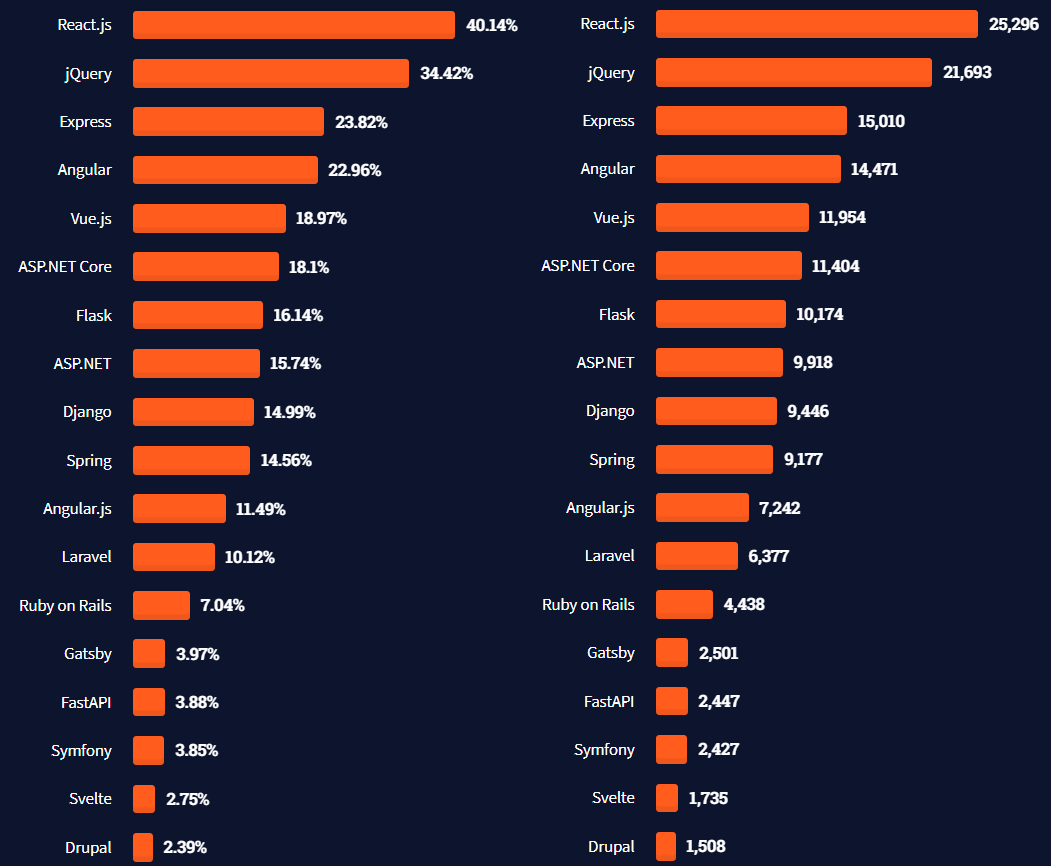
\includegraphics[scale=0.5]
    {Most popular Web Frameworks [Both] 2021.png}
    \caption{ Which web frameworks and libraries have you done extensive development work in over the past year, and which do you want to work in over the next year? (If you both worked with the framework and want to continue to do so, please check both boxes in that row.) {\cite{SO01}}}

  \end{figure}
\end{flushleft}

\newpage

\begin{flushleft}
  \textbf{Github}\\
  GitHub ist die Plattform für die Versionskontrolle von Source-Code, wo mehr als 238 Millionen Repositories\footnote{Ablage wo Quellkode gespeichert wird} verwaltet werden{\cite{GH07}}.
\end{flushleft}

Die Anzahl der Repositories, in denen Code für Angular und, React gespeichert wird, gibt einen Hinweis auf die Beliebtheit dieses Frameworks.
\\
\begin{table}[h!]
  \centering
  \begin{tabular}{ |p{5cm}||p{3.6cm}|p{3.6cm}|  }
    \hline
    \multicolumn{3}{|c|}{Github Statistiken}                                                                                                  \\
    \hline
                                                                                                                   & Angular/core & React     \\
    \hline
    Anzahl von     Repositories                                                                                    & 2,011,663    & 7,868,546
    \\

    %& Vue: & 2,299,614
    %   \hline
    %  Offene Issues           & 1,716         & 321       & 634
    %  \\
    \hline
    Stars insgesamt \footnote{Stars werden auf Github verwendet, um die Beliebtheit eines Repositorys anzuzeigen.} & 77.2k        & 170k
    \\
    \hline
  \end{tabular}
\end{table}

{\cite{GH04, GH06}}%GH05,

%https://risingstars.js.org/2020/es#section-statemanagement
%https://www.freecodecamp.org/news/angular-react-vue/
\begin{flushleft}

\textbf{NPM Paketen}\\
NPM verwaltet die Abhängigkeiten eines Angular oder React Projekts.

Die Anzahl der heruntergeladenen NPM-Pakete gibt einen Hinweis auf die Nutzung der Technologie.
\end{flushleft}

\begin{center}
  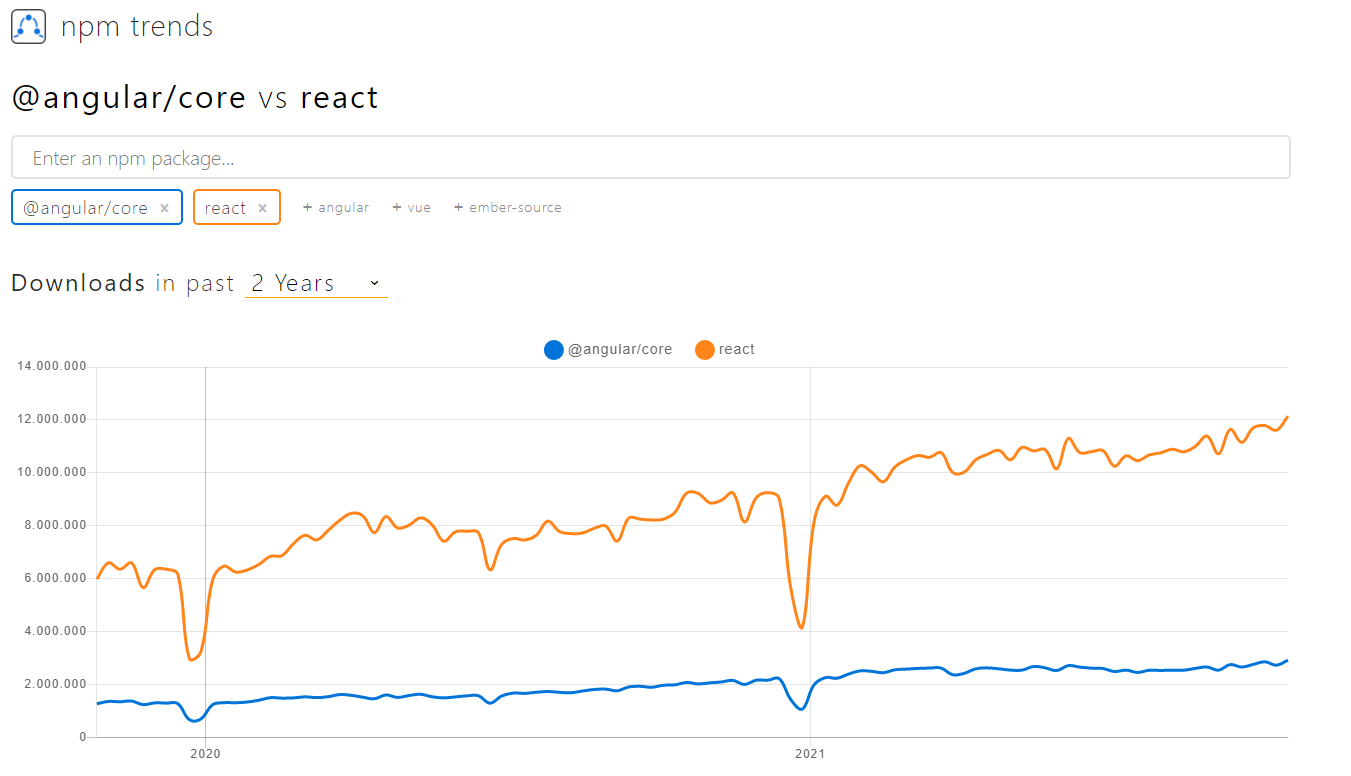
\includegraphics[scale=0.4]
  {sources/NPM-Trends React_Angular}\label{fig:NPM-Trends React_Angular}\\
  \textbf{Abbildung \autoref{fig:NPM-Trends React_Angular}:} heruntergeladenen NPM-Pakete \\@angular/core vs react
    {\cite{NPM01}}
\end{center}

\newpage

\begin{flushleft}
\textbf{Google Trends}\\
Laut Google Trends war React zwischen 01.11.2020 und 26.10.2021 das am häufigsten konsultierte Frontend Technologie in Deutschland.
\\
Diese Metrik ist ein weiterer Aspekt für die Beliebtheit von Framework.
\end{flushleft}

\begin{center}
  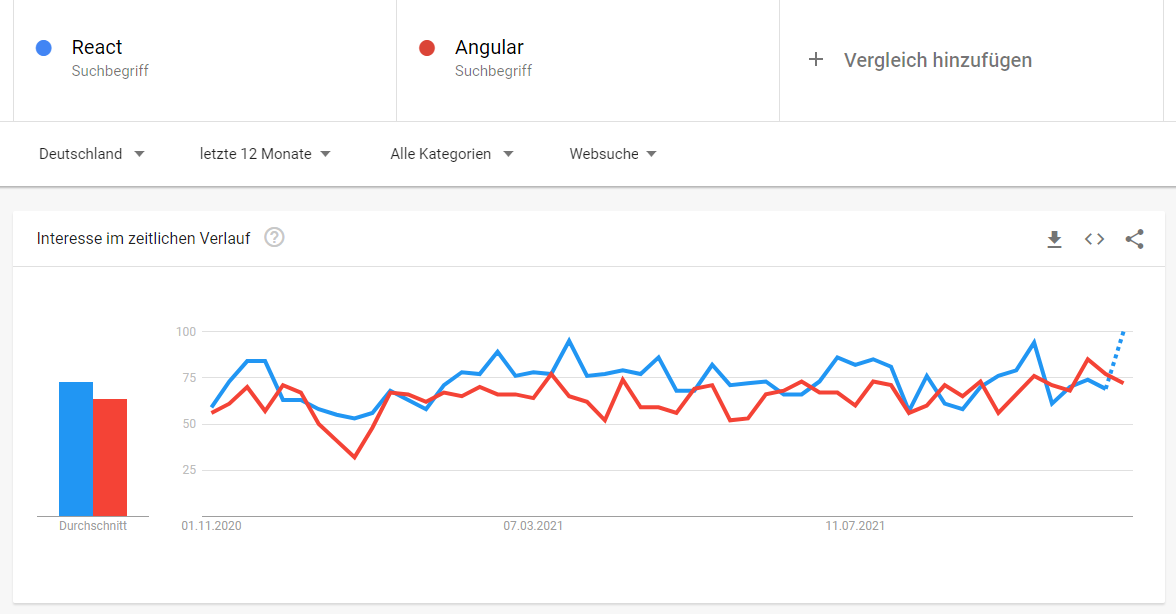
\includegraphics[scale=0.5]
  {sources/GoogleTrends React Angular 1.11.2020 29.10.2021}\label{fig:GoogleTrends React Angular 1.11.2020 29.10.2021}\\
  \textbf{Abbildung \autoref{fig:GoogleTrends React Angular 1.11.2020 29.10.2021}:} Google Trends Angular vs React
    {\cite{GO01}}
\end{center}

\begin{flushleft}
\textbf{Jobangebote}\\
Als angehende Informatiker sind berüfliche Perspektiven relevant, deswegen wurde den Arbeitsmarkt in der Entscheidungsfindung berücksichtigt.
\\
%In der Entscheidungsfindung sind ebenfalls künftige Perspektiven relevant.
%Aus diesem Grund ist als angehende Informatiker den Arbeitsmarkt berücksichtigt.    
  Anzahl der Jobangebote bei LinkedIn in Deutschland:
  \\
  Angular: 7.657 Ergebnisse{\cite{LI1}}
  \\
  React: 11.523 Ergebnisse{\cite{LI2}}
  %\\
  %Vue: 2.800 Ergebnisse{\cite{LI1}}
\end{flushleft}
AB HIER ÜBERARBEITEN:

\subsection{Framework vs Bibliothek}
\begin{flushleft}
In dieser Arbeit stehen ein Framework und eine Bibliothek zur Auswahl.
\\
Beide Technologien wurden für die Entwiklung von SPAs\footnote{Single-page application {\cite{MO1}}} konzipiert.

Eine Bibliothek wie React bietet mehr Kontroll darauf, wie der Code entwickelt werden kann und erlaubt die Applikation mit anderer Bibliotheken zu erweitern. Für das State-Management wird zum Beispiel häufig Redux{\cite{RE1}} verwendet.

Andererseits das Framework von Angular gibt genauer vor, wie der Code entwickelt werden muss.
\\
In dieser Arbeit wird nicht näher auf den Unterschied zwischen einer Bibliothek und einem Framework eingegangen, da beide die Anforderungen des Projekts abdecken.
\end{flushleft}

\subsection{Angular}
Angular ist das Framework von Google für Mobil- und Webanwendungen.

Angular hat eine steile Lernkurve im Vergleich zu React.{\cite{E01}}, S.25.
\\
%STIMMT DAS? Angular lässt weniger Spielraum für eigene Entscheidungen darüber, wie der Code entwickelt wird. Deshalb eignet sich Angular besser für Projekte, wo mehrere Entwickler zusammenarbeiten. 

%Der Code wird mit Angular nach der Ri in einer vorgegebenen Art geschrieben werden sollte, um Einheitlichkeit zu schaffen.

Zu beachten ist, dass Angular nicht JavaScript als Hauptprogrammiersprache verwendet, sondern TypeScript. Dies bedeutet zusätzlichen Aufwand für das Erlernen des Frameworks. Dieses Framework ist besonders geeignet für fortgeschrittene, umfangreiche Projekte.
QUELLE?

%Angular ist ein komplexeres Framework als React.

%CHECK THIS
%https://merehead.com/blog/angular-vs-react-vs-vue-best-choice-2022/

%Google or Facebook on the other side can almost ensure a long-term commitment both in terms of active development and nancial aspects to their respective frameworks. S.59

%PASSENTHES KAPITELTHEMA´?


\subsection{React}
Bei der endgültigen Entscheidung wurden React aufgrund ihrer geringen Lernkurve, ihrer guten State Management, ihre große Popularität und ihrer Einfachheit berücksichtigt.
\\
React besteht aus rund 56.162 professionellen Entwicklern auf der ganzen Welt.
Laut einer StackOverFlow Umfrage hat React.js im Jahr 2021 jQuery als das am häufigsten verwendete Web-Framework überholt. {\cite{SO01}}
\\
Die Entscheidung fiel für React aufgrund der Vorkenntnisse des Entwicklerteams und der Anzahl an Jobangeboten.

%Die Entwicklung mit Angular hätte mehr Zeit und Lernaufwand gekostet. Außerdem ist das Projekt nicht komplex genug, um das Angular-Ökosystem zu benötigen.

\subsubsection{Nachteile}
%Bei der Auswahl des Frameworks wollten wir so unvoreingenommen wie möglich sein, daher listen wir einige Aspekte auf, die bei Projekten mit React zu beachten sind.

\subsection{React Hooks}
%https://www.javatpoint.com/react-hooks
Beginnend mit 16.8.0, enthält React eine stabile Implementierung von React Hooks.

Ab dieser Version wird React empfohlen, keine Klassen mehr für die Erstellung von Komponenten zu verwenden.
Mit Klassen geschriebene Komponenten werden weiterhin unterstützt und müssen nicht neu geschrieben werden.
  {\cite{R05}}

\textbf{useState}
Der Hook useState bietet die Möglichkeit an, den Zustand einer Anwendung zu verwalten. Sie besteht aus mindestens einen Wert (value) und einer Funktion (updateValue), die den Wert aktualisiert.
%Der Wert kann ein Zahl, ein String, ein Array oder sogar ein Objekt sein.
%Optional kann ein Anfangswert (initialValue) definiert werden.

In unserem Projekt wurde useState verwendet, um alle Benutzerdaten zu manipulieren und dem Benutzer anzuzeigen.

Diese Benutzerdaten sind die Antwort auf die an den Server gesendete Abfrage.
Ein Beispiel von einer Server-Antwort befindet sich im Anhang 1.
Eine genauere Funktionsweise der Serverabfragen folgt in Kapitel Serverabfragen.
\\
%In späteren Kapiteln wird näher erläutert, wie diese Informationen, die durch einen einzigen Abfrage an den Server erhalten werden, in den Chat- und Benutzerkomponenten genutzt werden.

%Wie man sieht, gibt es innerhalb des states nicht nur einen Wert, sondern mehrere.
%Es handelt sich eigentlich um ein Objekt. Objekte sind dasselbe wie Variablen in JavaScript, der einzige Unterschied ist, dass ein Objekt mehrere Werte in Form von Eigenschaften und Methoden enthält.
%Objekte können andere Objekte, Strings, Arrays, Zahlen und so weiter enthalten.
\newpage

\textbf{useEffect}
useEffect ermöglicht es, verschiedene Arten von Effekten zu erzeugen, nachdem eine Komponente gerendert wurde.

Unter anderem ist mit useEffect folgenden möglich:\\\\
\\-Aktualisieren des DOM,
\\-Abrufen und Konsumieren von Daten von einer Server-Schnittstelle,
\\-Einrichten eines Abonnements, usw.
%https://www.javatpoint.com/react-hooks
\\
\begin{flushleft}
  %  Der Hook useEffect entspricht einer Kombination aus componentDidMount, componentDidUpdate und componentWillUnmount.

  Bei diesem Projekt wird die Anzeige der Daten abhängig der Änderungen des lokalen Zustands manipuliert.
\end{flushleft}

Im Bereich Profil werden die Änderungen erstmal zwischengespeichert, bevor sie in der Datenbank gespeichert werden.
\\
Die Abfrage zur Aktualisierung der Daten wird in dem Moment an den Server gesendet, in dem der Benutzer auf die Taste „Save/Speichern“ drückt.
\\
Zu diesem Zeitpunkt wird die Benutzeroberfläche durch useEffect aktualisiert, da sich eine der Abhängigkeitsvariablen geändert hat.
%\\
%Der globale Zustand „state“ ist in der Komponente App enthalten.
%In diesem wird die Antwort von der Datenbankenabfrage gespeichert.
%Wir definieren den Zustand als Abhängigkeit von useEffect, so dass er bei jeder Änderung in der Benutzeroberfläche aktualisiert wird.
\\

\begin{flushleft}
  Es ist möglich, mehrere useEffects zu einstellen und mit ihrer jeweiligen Abhängigkeiten separat definieren.
  Wenn es erfordelich ist, dass der Code innerhalb dem useEffect nur einmal nach dem ersten Rendering(deutsches WORT) ausgeführt wird, muss ein leeres Array als Abhängigkeit definiert werden.
\end{flushleft}

%WELCHES PROBLEM HABEN WIR DAMIT GELÖST?  

\textbf{useContext}
useContext ermöglicht Daten innerhalb bestimmte Komponenten zu teilen.

In diesem Projekt war useContext eingesetzt, um die Benutzerdaten und den Authentifizierungstoken über die Komponenten  „Profile“, „Chat“, „Users“ (to swipe) zu teilen.
\\
In frühen Versionen des Projekts wurde für den gleichen Zweck props verwendet.  {\cite{R03}}
UseContext bietet eine weitere Lösung, um Daten zwischen Komponenten auszutauschen.{\cite{R04}}
\\

Im Anhang 5 und 6 befidet sich der Code mit dem den Authentifizierungstoken und die Benutzerdaten global  mithilfe von useContext verwaltet wird.

\subsection{Fazit}
Es ist anzumerken, dass die Entwicklung des Projekts mit jedem der beiden Frameworks möglich war.
...